\section{Adaptive-precision ADC Design}\label{architecture}

In this section, the proposed adaptive-precision ADC design is presented. Targeting the image processing applications, we choose to infuse adaptive-precision conversion capabilities into the SS and SAR/SS ADCs. The basic modules of the two ADC designs is overviewed firstly in \ref{over1} and \ref{over2}. Then, after showing the power gating implementation in \ref{gating1}, the adaptive-precision tuning within the SS and SAR/SS ADCs is specifically described in \ref{gating2} and \ref{gating3}, with the following architectural enhancements:

\begin{enumerate}[\IEEEsetlabelwidth{3)}]
	\item 
	The thermometer-code counter in the SS ADC has been extended to support two modes for adaptive-precision conversion, which can also provide an exponential long time for power gating.
	\item
    Stability-optimizing switches are inserted into the comparators in the SS ADC to avoid unpredictable latch for low-precision conversion results due to comparators' power off. 
    \item
    Additional control signals in the SAR/SS ADC are carefully reused and effectively minimized, enabling effective power-scaling capabilities with little control circuit costs but some shared level-shifters and inverters.      
\end{enumerate} 


%For other ADCs of different architecture, the proposed method can also be adopted.

\subsection{SS ADC Architecture Overview}\label{over1}

The overall architecture of the SS ADC is presented in Fig.~\ref{SSADC}. The main modules include column-parallel Correlated Double Sampling (CDS) circuits, comparators, 
and a column-shared ramp generator. Fig.~\ref{SSWAVE} shows the basic operational waveform of the SS ADC. At the time when the ramp signal exceeds the output of a CDS circuit in a certain column, 
the corresponding comparator will be flipped and latch the time information $\Delta t$ into the following 8-bit latch as the conversion results. 
Such conversions across all columns will be done as soon as the ramp signal reaches $V_{refh}$.

\begin{figure}[htbp]
	\centerline{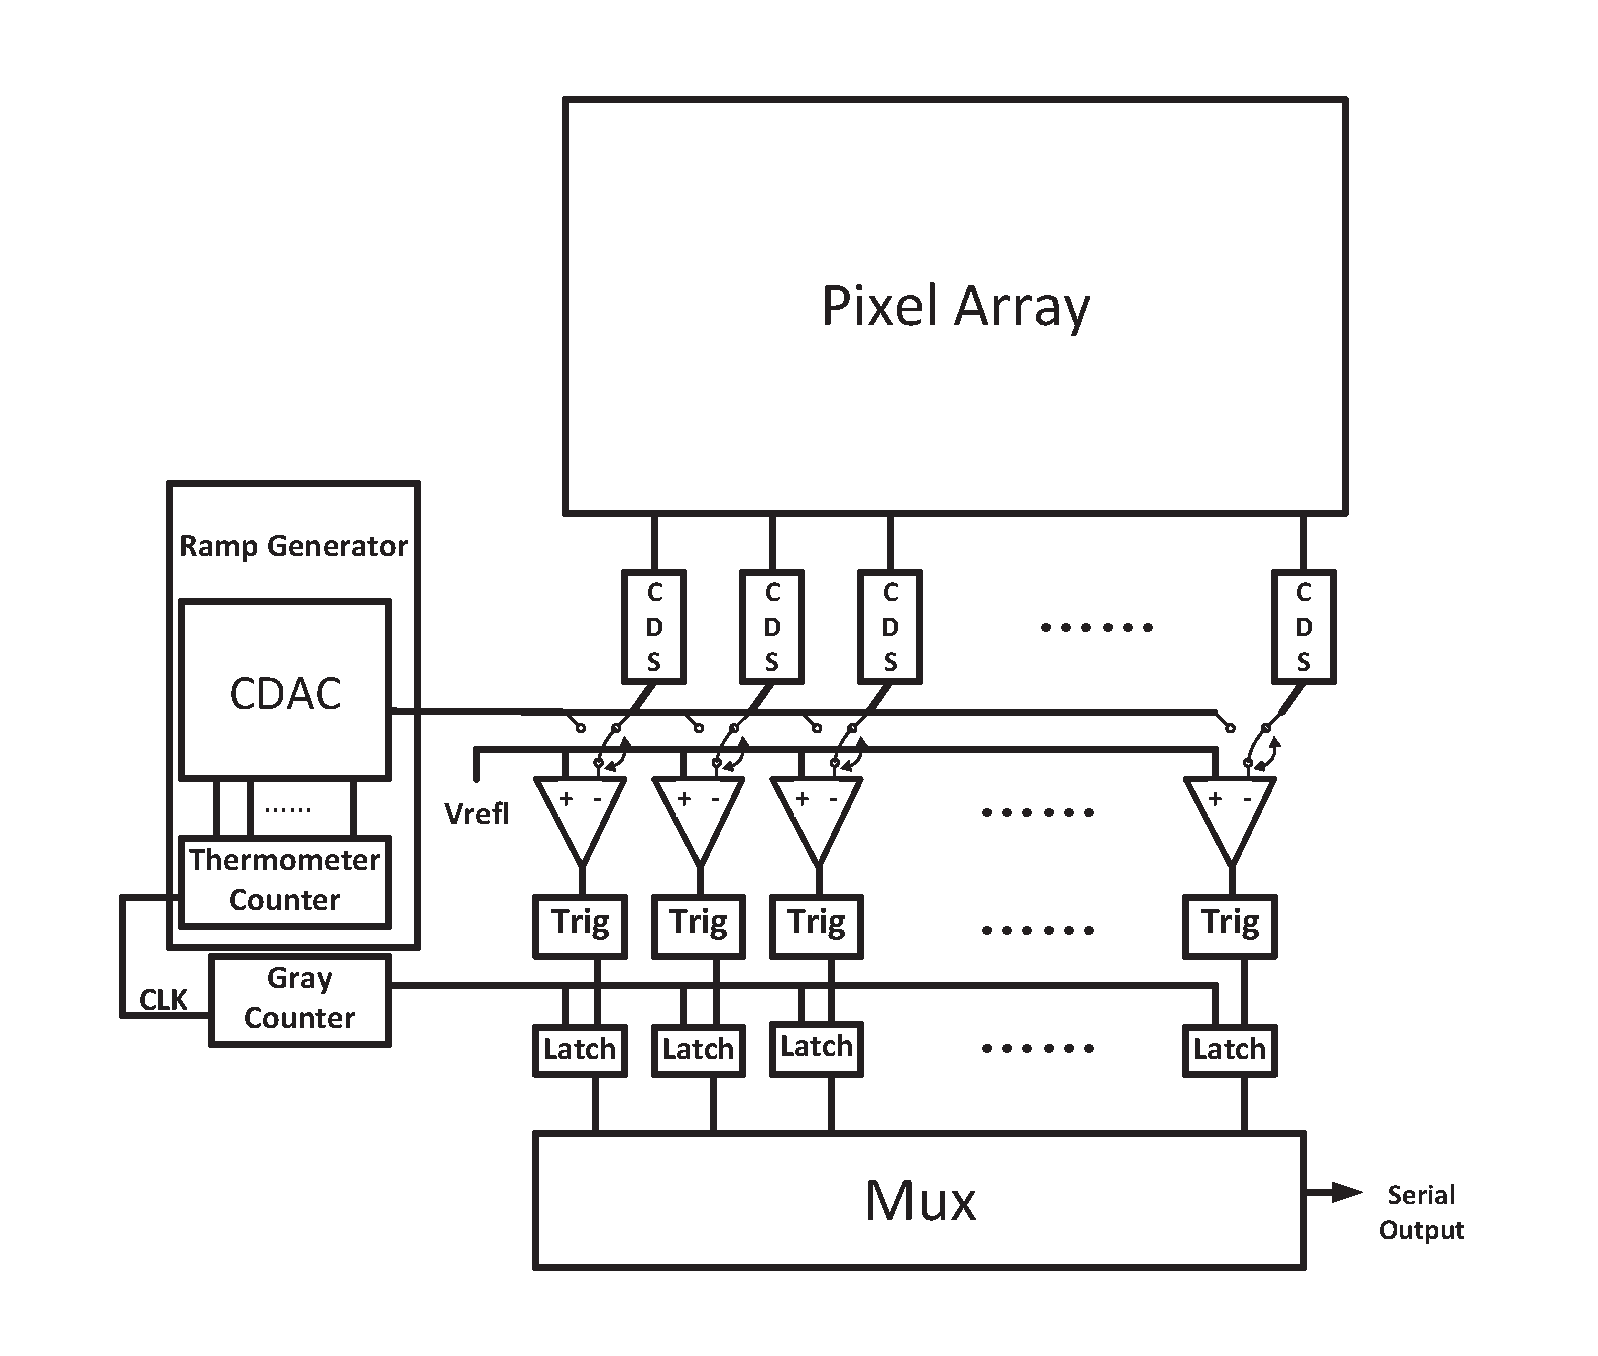
\includegraphics[width=3.5in]{./Figures/SSADC.eps}}
	\caption{Overall architecture of the SS ADC.}
	\label{SSADC}
\end{figure} 

\begin{figure}[htbp]
	\centerline{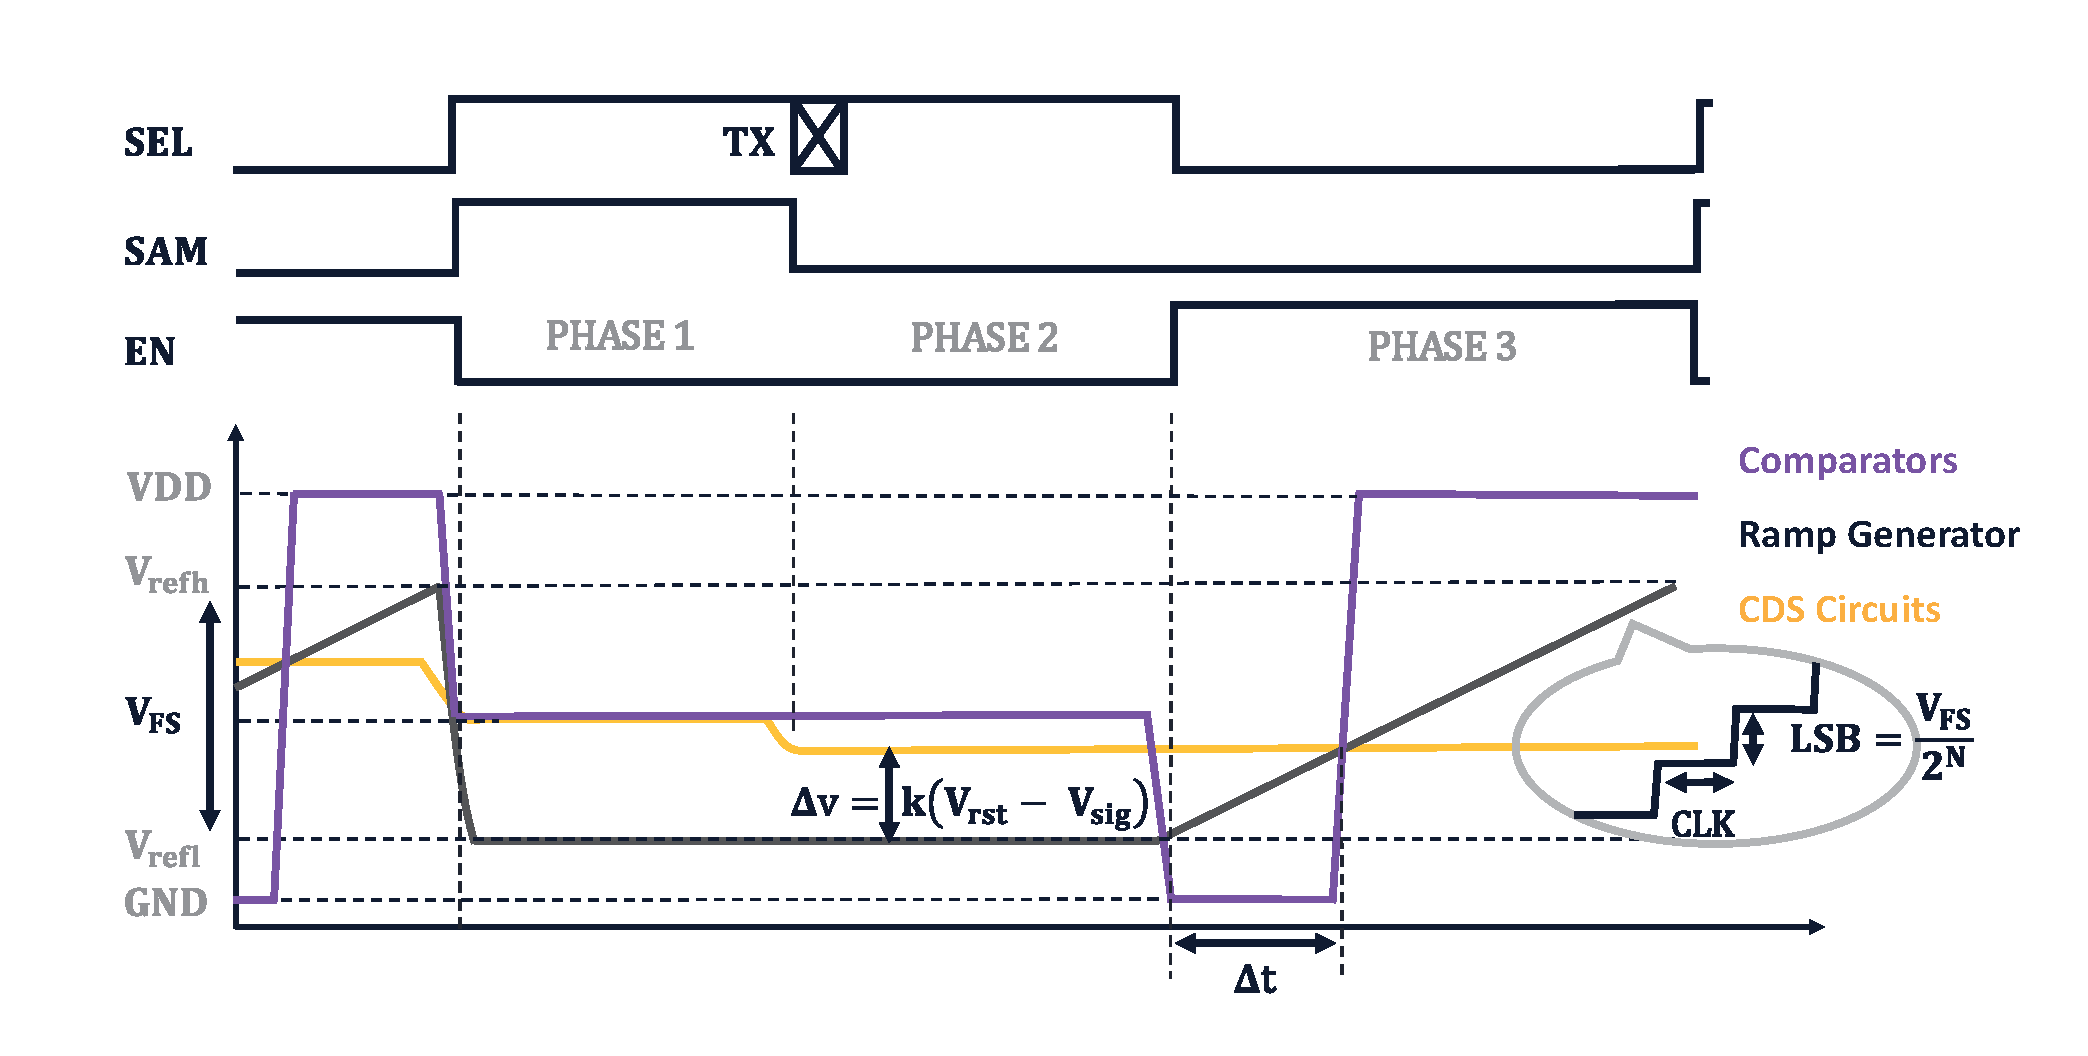
\includegraphics[width=3.5in]{./Figures/SSWAVE.eps}}
	\caption{Operational waveform of the SS ADC.}
	\label{SSWAVE}
\end{figure}

As the structure of the three main modules are described more specifically below, details of the three waves in Fig.~\ref{SSWAVE} are also revealed.

\subsubsection{CDS Circuits}

CDS circuits are the interface between the pixel array and the ADC, responsible for subtracting the pixels’ signal voltages from reference voltages and 
amplifying the difference by a certain coefficient. The difference (i.e. $\Delta{V}$ in Fig.~\ref{SSWAVE}) is physically attached to the exposure time of the pixels, 
and the subtraction will help remove the noise caused by the varying reference voltages. 

Switched-capacitor operational amplifiers are commonly used in CDS circuits as presented in Fig.~\ref{CDS}. According to the law of charge conservation, 
the output voltage of the CDS circuits (in PHASE2 of Fig.~\ref{SSWAVE}) can be calculated as \eqref{eq1}, consistent with the requirements. It is also noticed that the Input Offset Cancelation (IOS) is realized \cite{razavi_design_1992}, 
which is necessary because the amplifiers in different columns may have different offset voltages.

\begin{figure}[htbp]
	\centerline{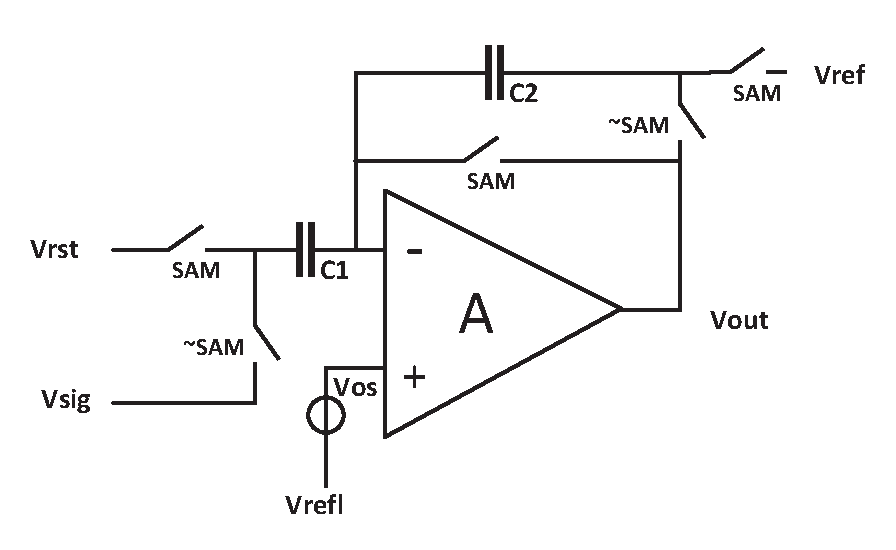
\includegraphics[width=2.5in]{./Figures/CDS.eps}}
	\caption{The structure of the CDS circuits.}
	\label{CDS}
\end{figure} 

\begin{equation}
	\begin{aligned}
		V_{out}&=\left[ V_{ref}+\frac{C_1}{C_2}\ast\left(V_{rst}-V_{sig}\right)\right]\ast\frac{\beta A}{1+\beta A}\\
		&\;{+}\;\left(V\right._{refl}+V_{os})\ast\frac{A}{1+A}\ast\frac{1}{\beta A}\\
		&\;where\ \ \beta=\frac{C_2}{C_1+C_2}
		\label{eq1}
	\end{aligned}
\end{equation}

\subsubsection{Ramp Generater}

As presented in Fig.~\ref{RAMP}, the ramp generator in the SS ADC consists of a thermometer-code counter and a Capacitor Digital-to-Analog Converter (CDAC). 
While the capacitors in CDAC are being switched one by one from $V_{refl}$ to $V_{vefh}$, the output voltage of the ramp generator is expressed as \eqref{eq2} according to the law of charge conservation. 
In this equation, $N$ represents the number of switched capacitors and $M$ represents the total number of capacitors with the same size (for the 8-bit precision, the total number will be 255). 
Therefore, as in PHASE3 of Fig.~\ref{SSWAVE}, the ramp signal will be like stages from $V_{refl}$ to $V_{refh}$, of which the range matches the output of CDS circuits. 
And the height of each stage is actually the Least Significant Bit (LSB) of the ADC conversion.

The three buffers in Fig.~\ref{RAMP} ensure that the reference voltages and ramp signal have sufficient driving capabilities, 
and the output buffer will be in the largest size since it has to drive hundreds of column-parallel comparators.

\begin{figure}[htbp]
	\centerline{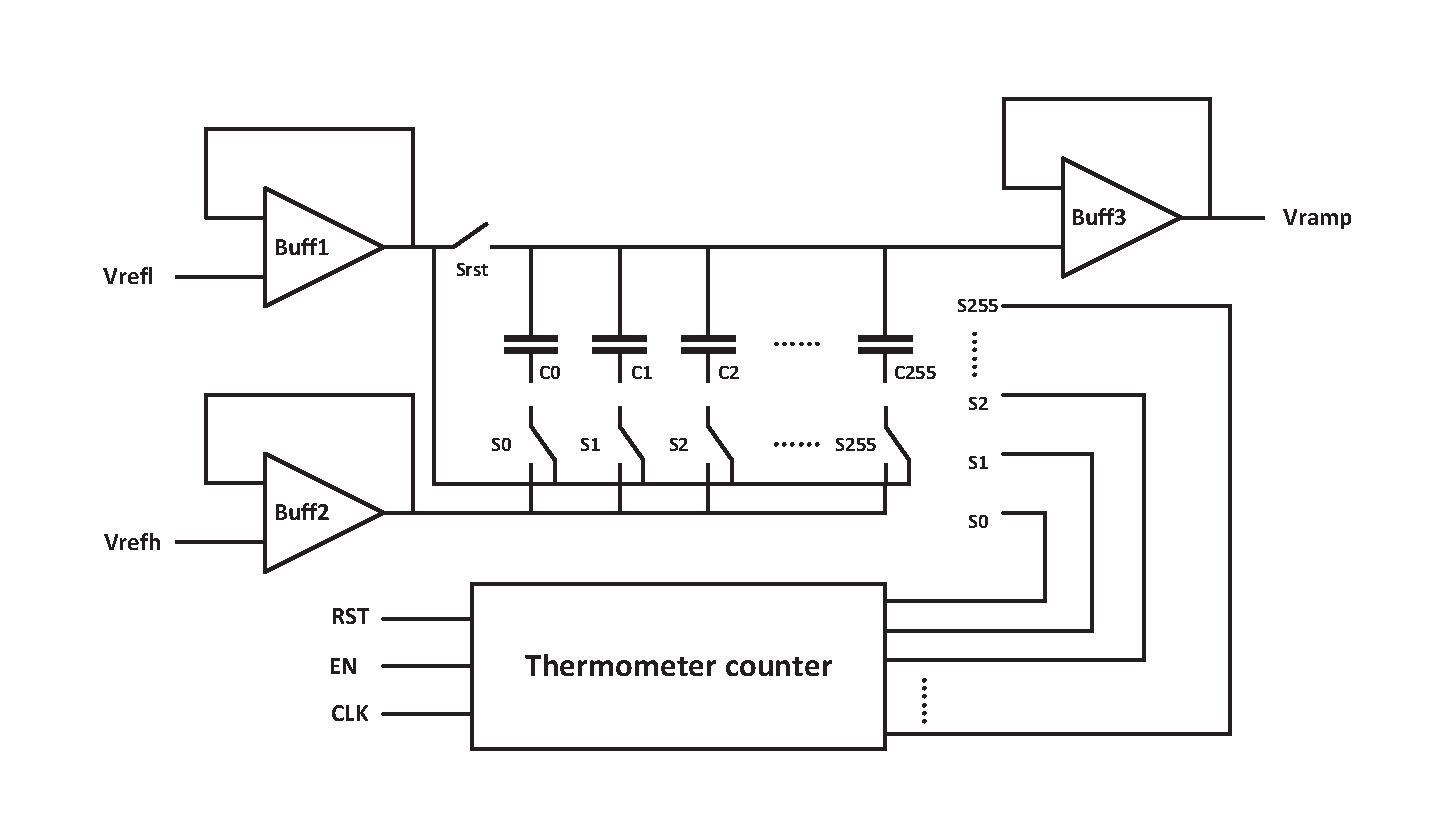
\includegraphics[width=3.5in]{./Figures/RAMP.eps}}
	\caption{The structure of the ramp generator in the SS ADC.}
	\label{RAMP}
\end{figure} 

\begin{equation}
	V_{ramp}=V_{refl}+\frac{N}{M}\ast\left(V_{refh}-V_{refl}\right)
	\label{eq2}
\end{equation}

\subsubsection{Comparators}

The comparators are used to compare the CDS circuits' output with the ramp signal from the ramp generator. 
In the SS ADC, two-stage open-loop comparators can be applied as presented in Fig.~\ref{COM}. According to the law of charge conservation, 
the comparators’ output (in PHASE3 of Fig.~\ref{SSWAVE}) can be computed as \eqref{eq3}. The comparison will be dominated by $V_{ramp}-V_{cds}$ as long as the amplifiers’ open-loop gain 
is large enough while the IOS is also realized.% In addition, the comparators’ speed relies on the bandwidth and slew rate of the amplifiers.

\begin{figure}[htbp]
	\centerline{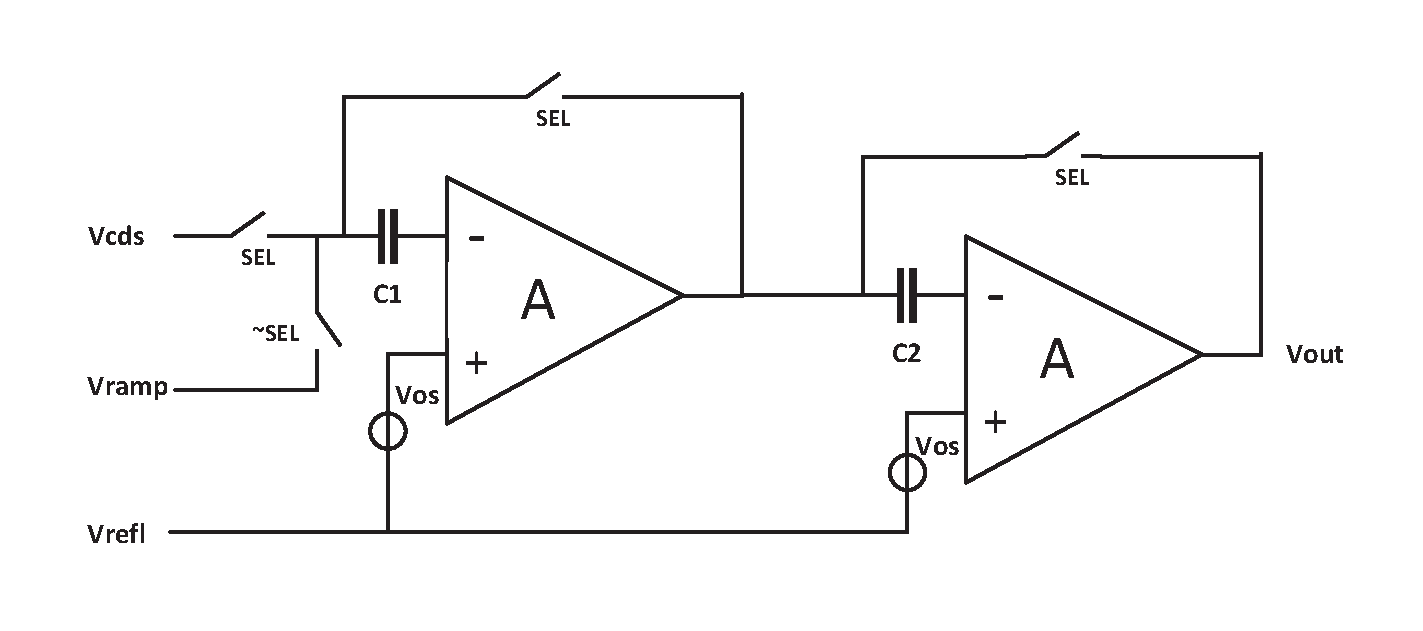
\includegraphics[width=2.5in]{./Figures/COM.eps}}
	\caption{The structure of the comparators in the SS ADC.}
	\label{COM}
\end{figure} 

\begin{equation}
	\begin{aligned}
		V_{out}&=A^2(V_{ramp}-V_{cds})\\
		&\;{+}\;\left(V_{refl}+V_{os}\right)\ast\frac{A}{1+A}\\ 		
		\label{eq3}
	\end{aligned}
\end{equation}

\subsection{SAR/SS ADC Architecture Overview}\label{over2}

%Fig.~\ref{SARADC} shows 
The overall architecture of the SAR/SS ADC is almost the same as the SS ADC in Fig.~\ref{SSADC}. The only two differences are that the comparators are replaced by low-precision (4bit) SAR sub-ADC and
the ramp generator is replaced by a Resistor Digital-to-Analog Converter (RDAC) with a onehot-code counter.

\iffalse
\begin{figure}[htbp]
  \centerline{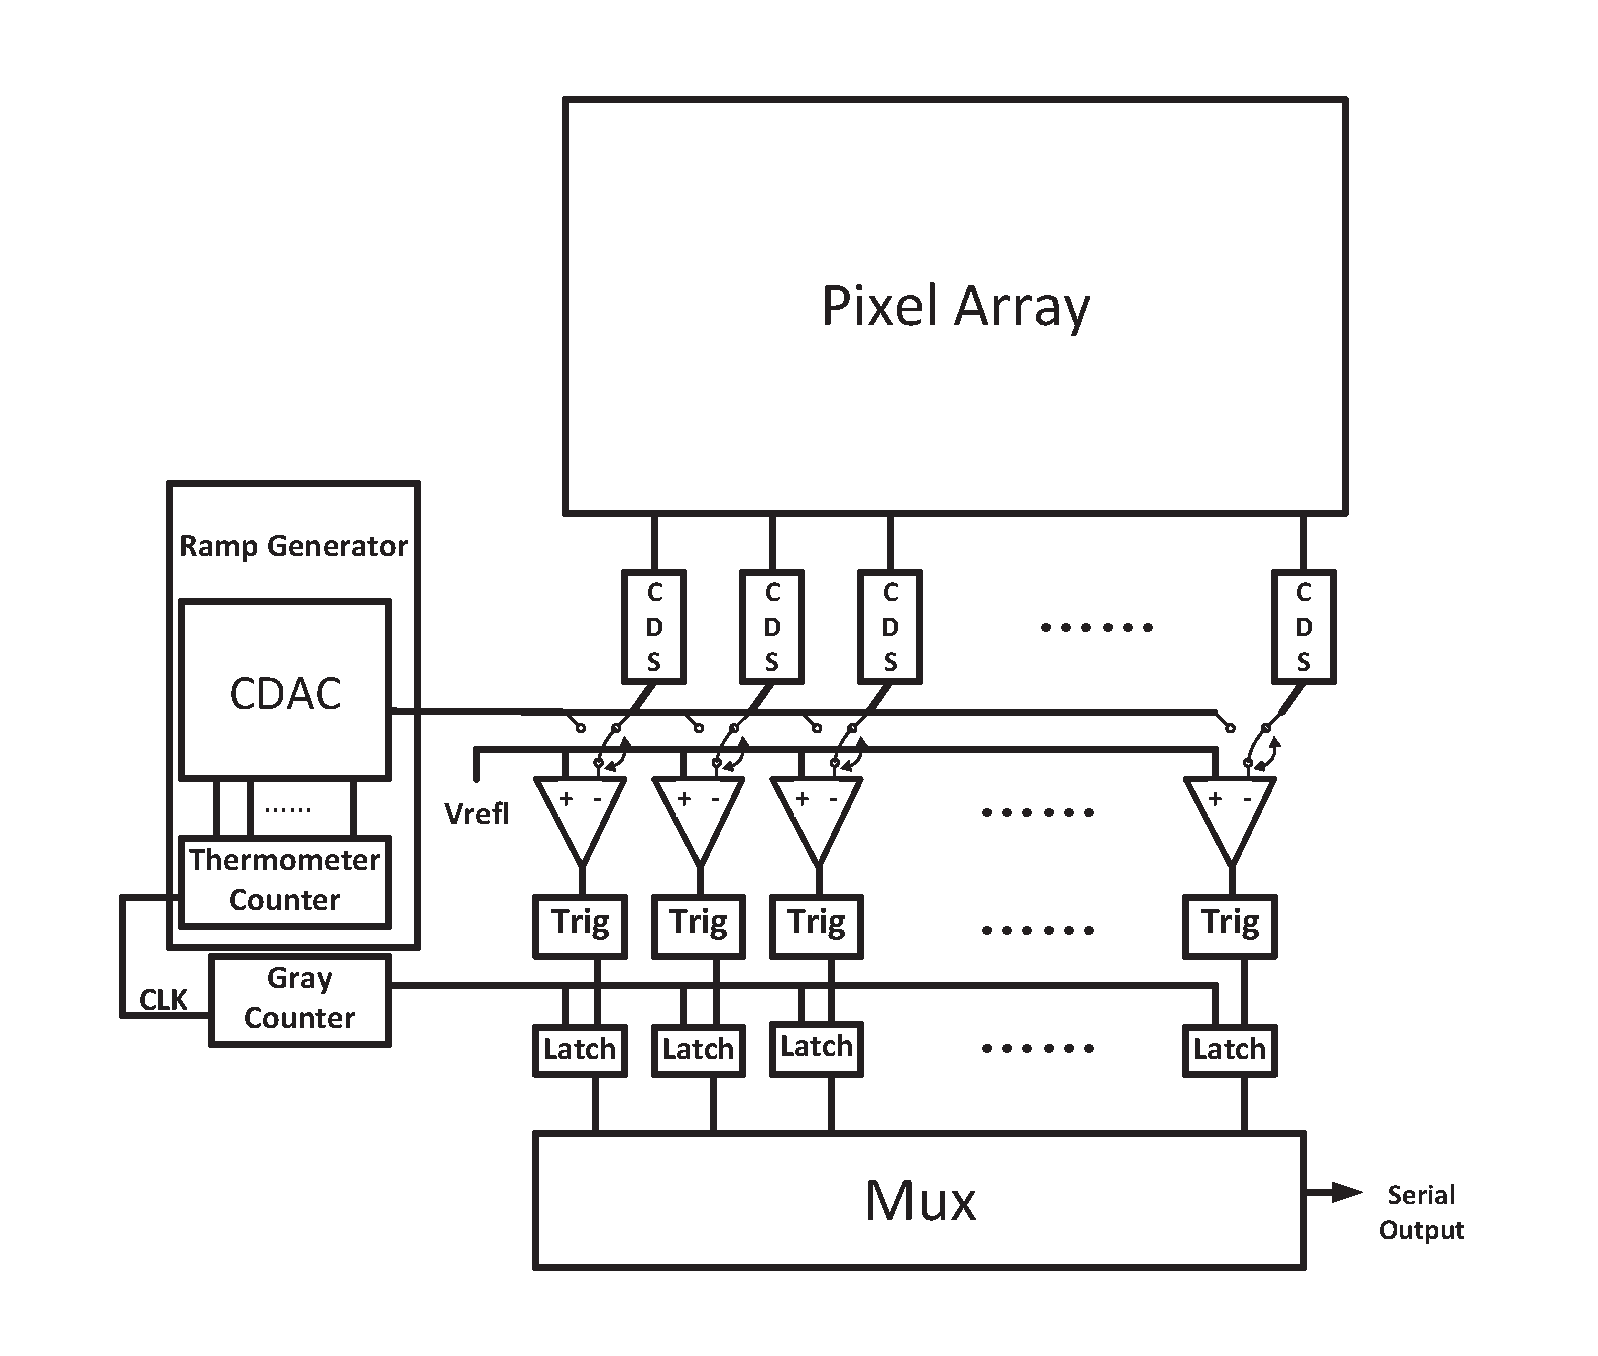
\includegraphics[width=3.5in]{./Figures/SARADC.eps}}
  \caption{Overall architecture of the SAR/SS ADC.}
  \label{SARADC}
  \end{figure}
\fi 

As presented in Fig.~\ref{SAR}, a SAR sub-ADC is composed of two input buffers of the reference voltages, an array of digital-to-analog capacitors, a dynamical comparator and a SAR logic block. While generating the upper 4-bit results, $V_{X}$ in the SAR sub-ADC will be changed according to the SAR logic. That means after 4 comparisons 
with the reference voltage, $V_{X}$ will be as \eqref{eq4}, where $D_{U}\left[\,i\,\right]$ is the $i$ th bit of the upper 4 bits. 
Then the ramp generator starts working, making $V_{X}$ increase gradually as \eqref{eq5}, where $D_{L}\left[\,i\,\right]$ is the $i$ th bit of the lower 6 bits. 
At the time when $V_{X.2}$ exceeds $V_{ref}$, the corresponding $V_{cds}$ is expressed as \eqref{eq6}, which can be represented by the 10-bit conversion results, exactly.

\begin{figure}[htbp]
	\centerline{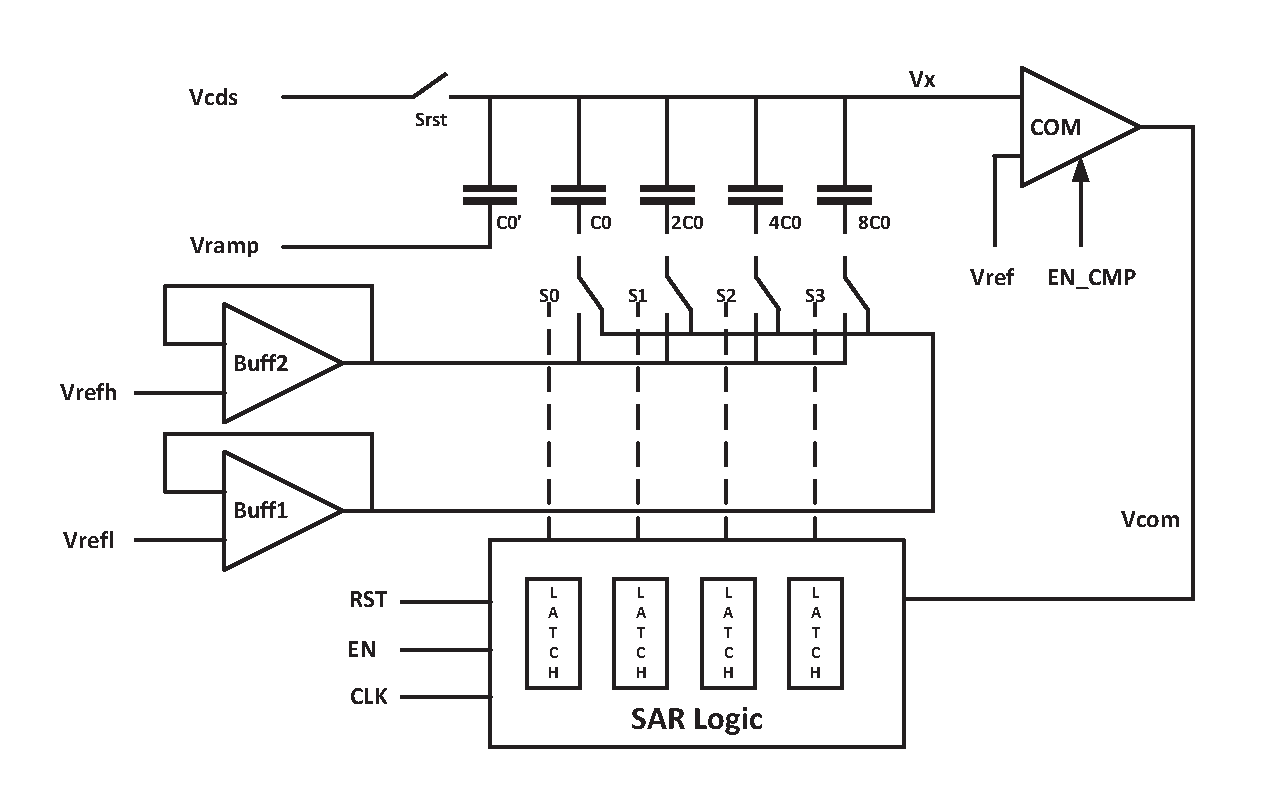
\includegraphics[width=3in]{./Figures/SAR.eps}}
	\caption{The structure of the SAR sub-ADCs in the SAR/SS ADC.}
	\label{SAR}
\end{figure}

\begin{equation}
	V_{X.1}=V_{cds}+\sum_{i=1}^{4} {\frac{V_{ref}}{2^{i}}\ast{D_{U}\left[\,i\,\right]}}
	\label{eq4}
\end{equation}

\begin{equation}
	\begin{aligned}
		&V_{X.2}=V_{X.1}+\frac{V_{ramp}}{2^4}\\ &where\  V_{ramp}=\frac{V_{ref}}{2^6-1}\ast\sum_{i=1}^{6}2^{6-i}\ast{D_{L}\left[\,i\,\right]}
		\label{eq5}
	\end{aligned}	
\end{equation}

\begin{equation}
	\begin{aligned}
		&V_{cds}=k\ast(V_{rst}-V_{sig})\\
		&\;{\approx}\;{V_{ref}-\sum_{i=1}^{4} \frac{V_{ref}}{2^{i}}\ast{D_{U}\left[\,i\,\right]}-\sum_{i=1}^{6} \frac{V_{ref}}{2^{4+i}}\ast{D_{L}\left[\,i\,\right]}}
		\label{eq6}
	\end{aligned}
\end{equation}

It is worth noting that we assign 14 steps for the 4 comparisons with SAR logic (in the SAR/SS ADC, we define 1 clock step as 2 clock periods, which is 100ns). Both the first and second comparison takes 4 steps and the following two comparison takes 3 steps. It is because that the more rapidly $V_{X}$ can be changed, the more time it may be required for comparison. As for the last comparison with SS logic, 1 step is sufficient because $V_{X}$ will not exceed $V_{ref}$ rapidly, allowing the comparators to response in-time.

Fig.~\ref{RRAMP} shows the structure of the ramp generator in the SAR/SS ADC, which consists of an R-string made up of 68 unit resistors. $V_{ramp}$ has a total number of 68 steps,
of which 64 steps with a step size of $(V_{refh}-V_{refl})/64$ are used to generate the lower 6-bit results and 4 redundant steps are used to ensure that the comparators 
will always be flipped to latch the results. In the working time, $V_{0}$ to $V_{67}$ in the ramp generator is sequentially selected as the output and thereby 
$V_{ramp}$ is changed from $V_{vefl}$ to $V_{vefl}+17/16(V_{refh}-V_{refl})$.

\begin{figure}[htbp] 
	\centerline{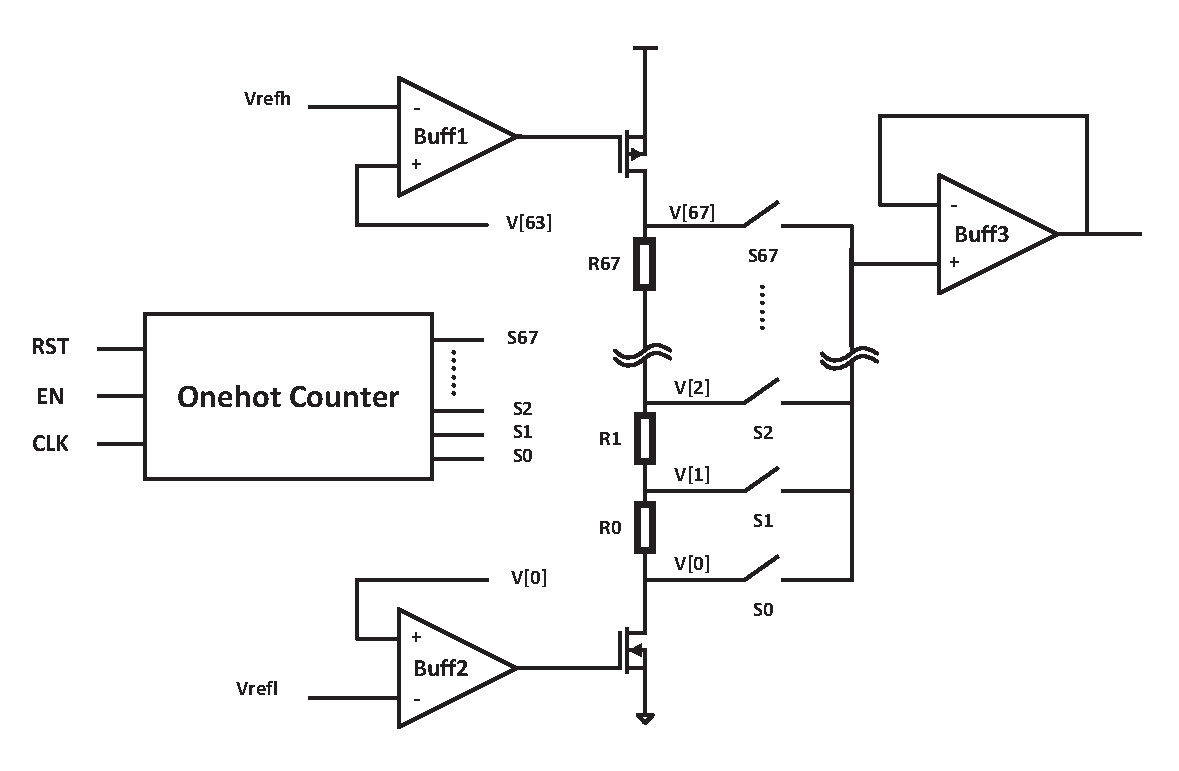
\includegraphics[width=2.5in]{./Figures/RRAMP.eps}}
	\caption{The structure of the ramp generator in the SAR/SS ADC.}
	\label{RRAMP}
\end{figure}

Compared to CDAC, RDAC is able to generate the ramp signal without the gain error caused by the input capacitors of the output buffer, 
which is necessary to achieve 10-bit precision in the SAR/SS hybrid architecture.
Besides, the two buffers of the reference voltages in the RDAC require less energy than those in the CDAC due to less load capacitance.  

The related operational waveform of the SAR/SS ADC is presented in Fig.~\ref{SARWAVE}. It is obvious that the upper 4-bit results (as the second last item of \eqref{eq6}) are generated 
with the SAR logic and the lower 6-bit results (as the last item of \eqref{eq6}) are counted according to the time between the ramp signal’s start and the comparators’ last flip. 

\begin{figure}[htbp]
	\centerline{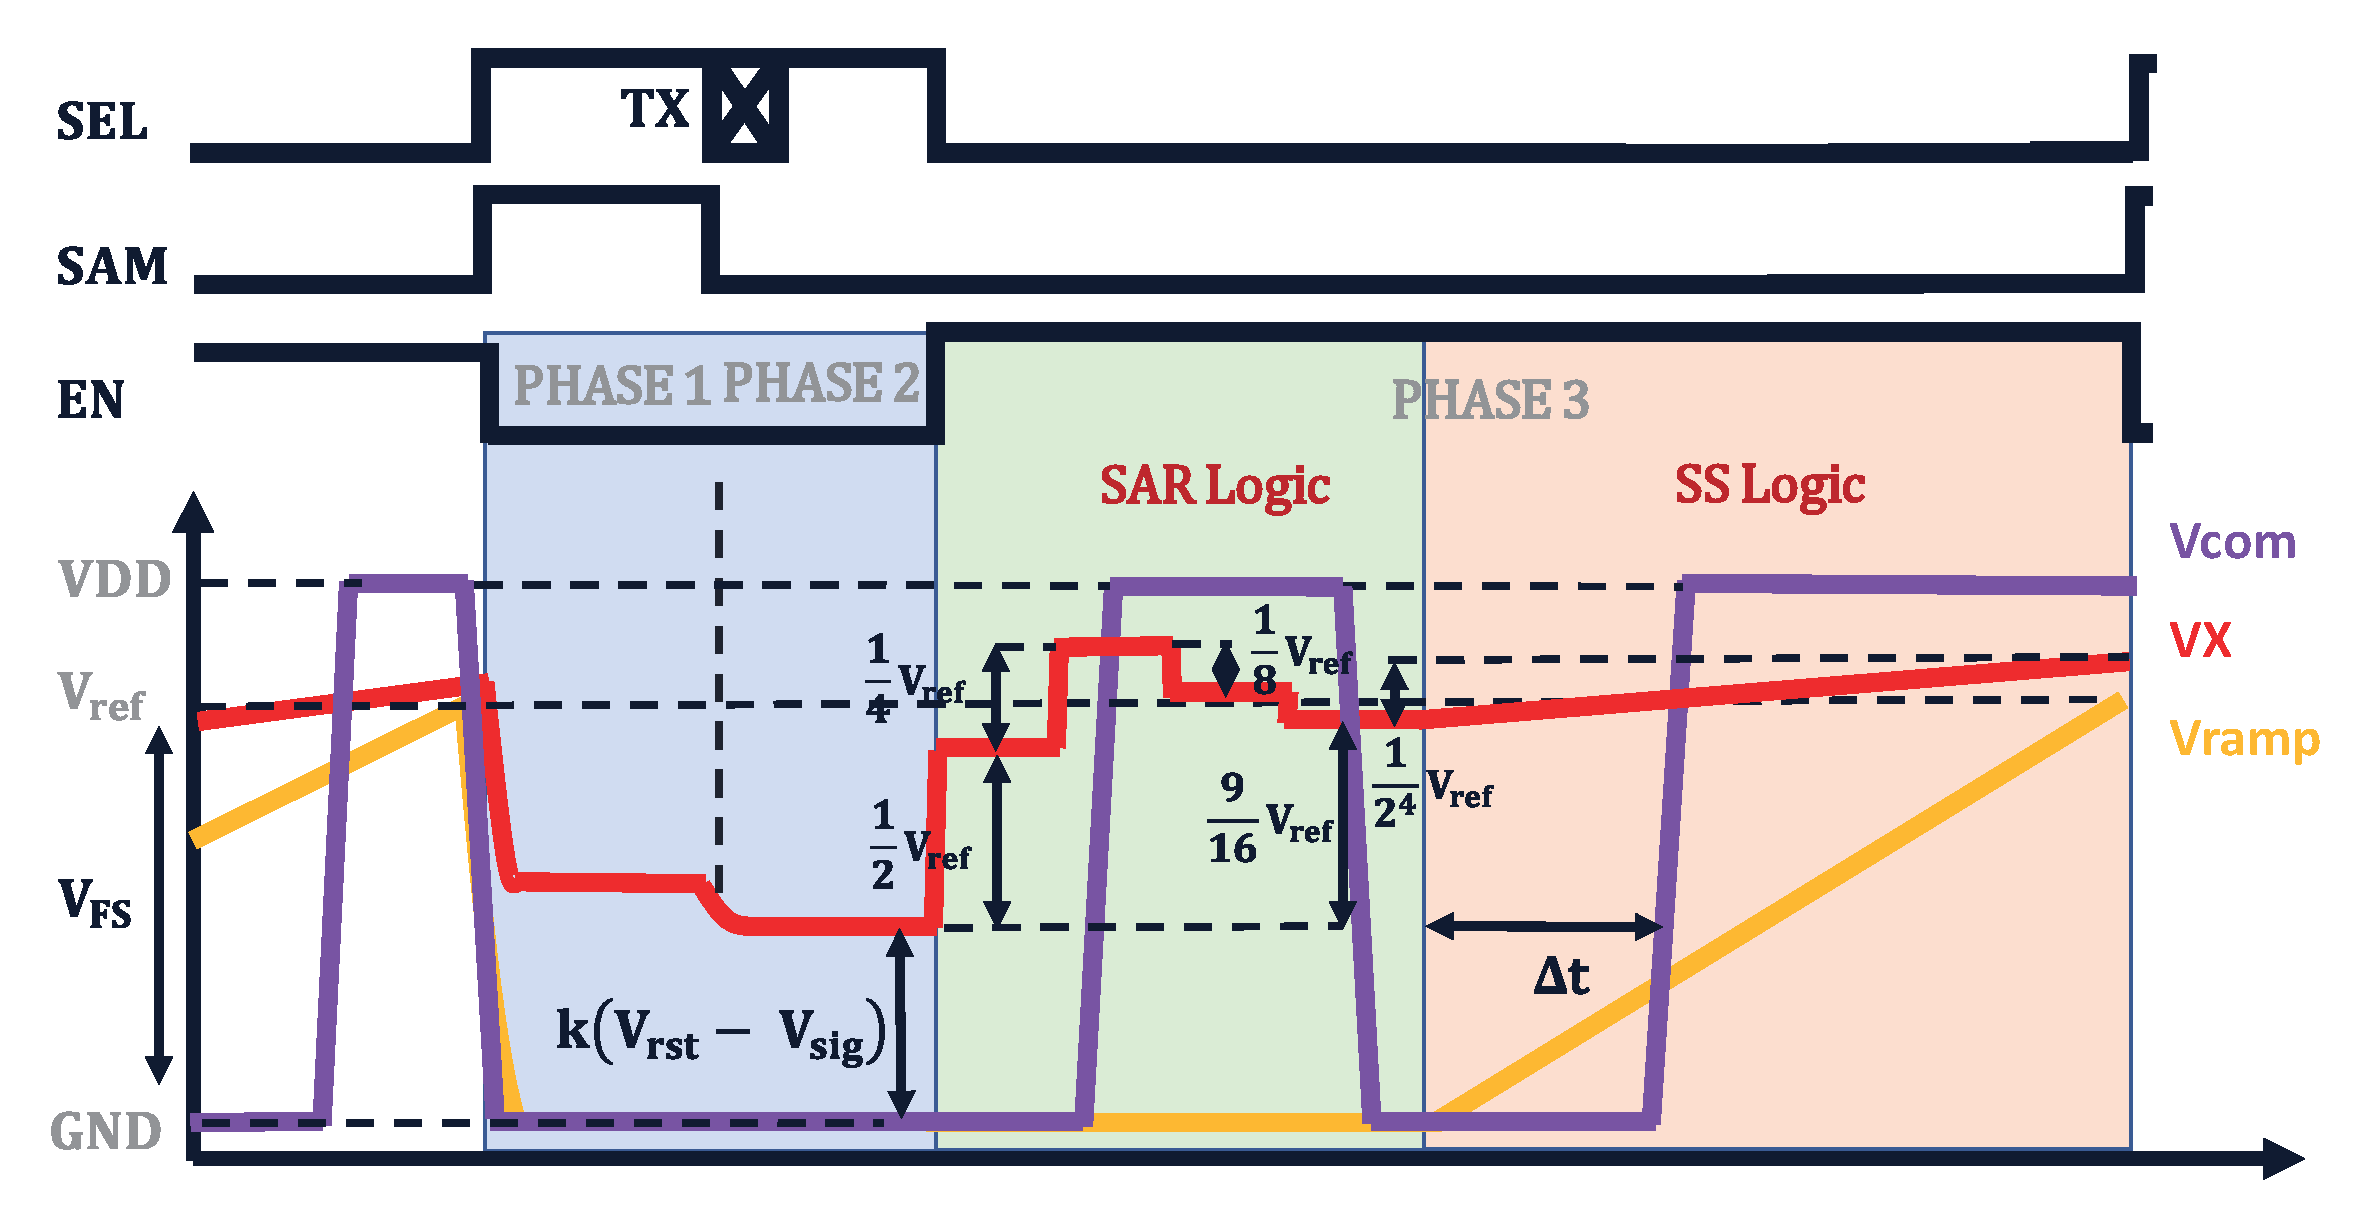
\includegraphics[width=3.5in]{./Figures/SARWAVE.eps}}
	\caption{Operational waveform of the SAR/SS ADC.}
	\label{SARWAVE}
\end{figure} 

As for the dynamical comparators inside the SAR sub-ADC, a traditional structure of a strong-arm comparator with pre-amplifiers can be used as presented in Fig.~\ref{LATCH}. Such comparators 
are suitable for multiple comparisons because high speed is easily achieved and every comparison is under the control of the clock. Besides, the offset voltages of the pre-amps can be effectively eliminated by Output Offset Cancelation (OOS) \cite{razavi_design_1992}.

\begin{figure}[htbp]
	\centerline{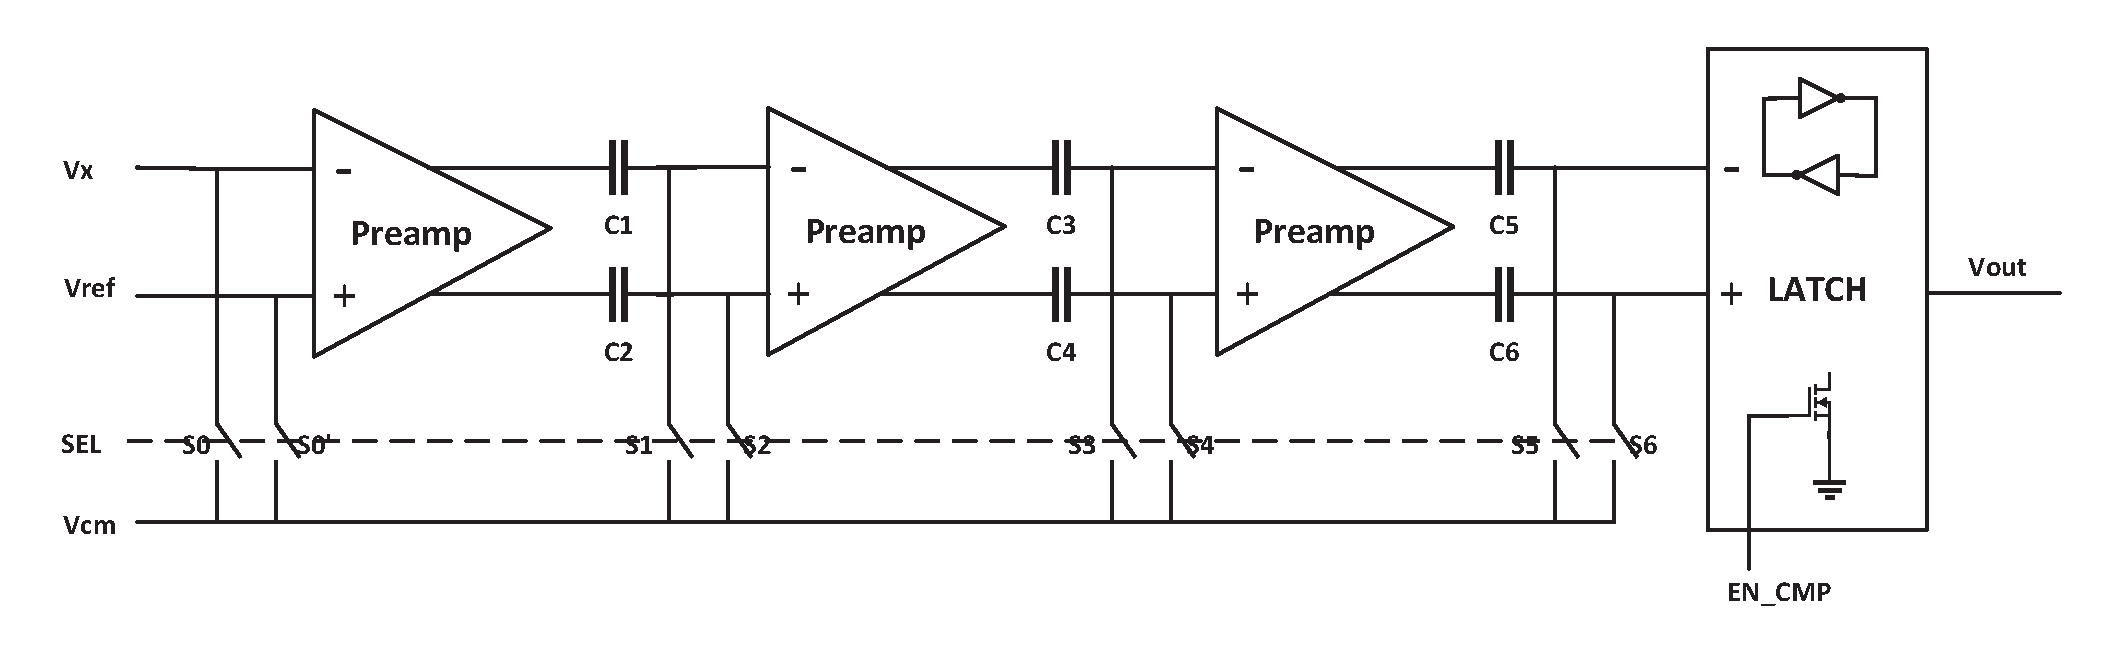
\includegraphics[width=3.5in]{./Figures/LATCH.eps}}
	\caption{The structure of the comparators in the SAR sub-ADCs.}
	\label{LATCH}
\end{figure} 

The reasons why we choose 4/8-bit adaptive-precision for the SS ADC and 4/10-bit adaptive-precision for the SAR/SS ADC are discussed in Sect.~\ref{discussion}.

%\subsection{Power Gating and Adaptive-Precision Implementation}\label{strategy}

\subsection{Implementation of Power Gating}\label{gating1}

The power gating can be implemented by adding PMOS-transistor switches between the functional blocks and the supply voltage \cite{keating_low_2007} as presented in Fig.~\ref{GATING}. 
When the switches are turned off, the corresponding blocks’ current paths will be cut off and thereby the energy is saved. 

It is obvious that for analog circuits, the more current is under control, the more effective the power gating can be. However, to avoid unacceptable IR drop, the total size of the switches may be large, 
and inverters should be inserted between the control signal and the switches’ gates for sufficient driving capabilities. 

Besides, the longer time the functional blocks can be power off, the better power scaling capacity can be obtained. And a continuous long time is preferred than separated short time for power gating because the blocks' shut-down and recovery time should also be taken into consideration.
As presented in Fig.~\ref{TIME}, separated short time for power gating will inevitably waste more
time due to the functional blocks' shut down and recovery. 

As the column-parallel ADCs not only have large amounts of column-parallel current that can be controlled, but also offer continuously and exponentially long power-off time thanks to the widely adopted SS conversion logic, applying power gating to this architecture will be highly efficient.

\begin{figure}[htbp]
	\centerline{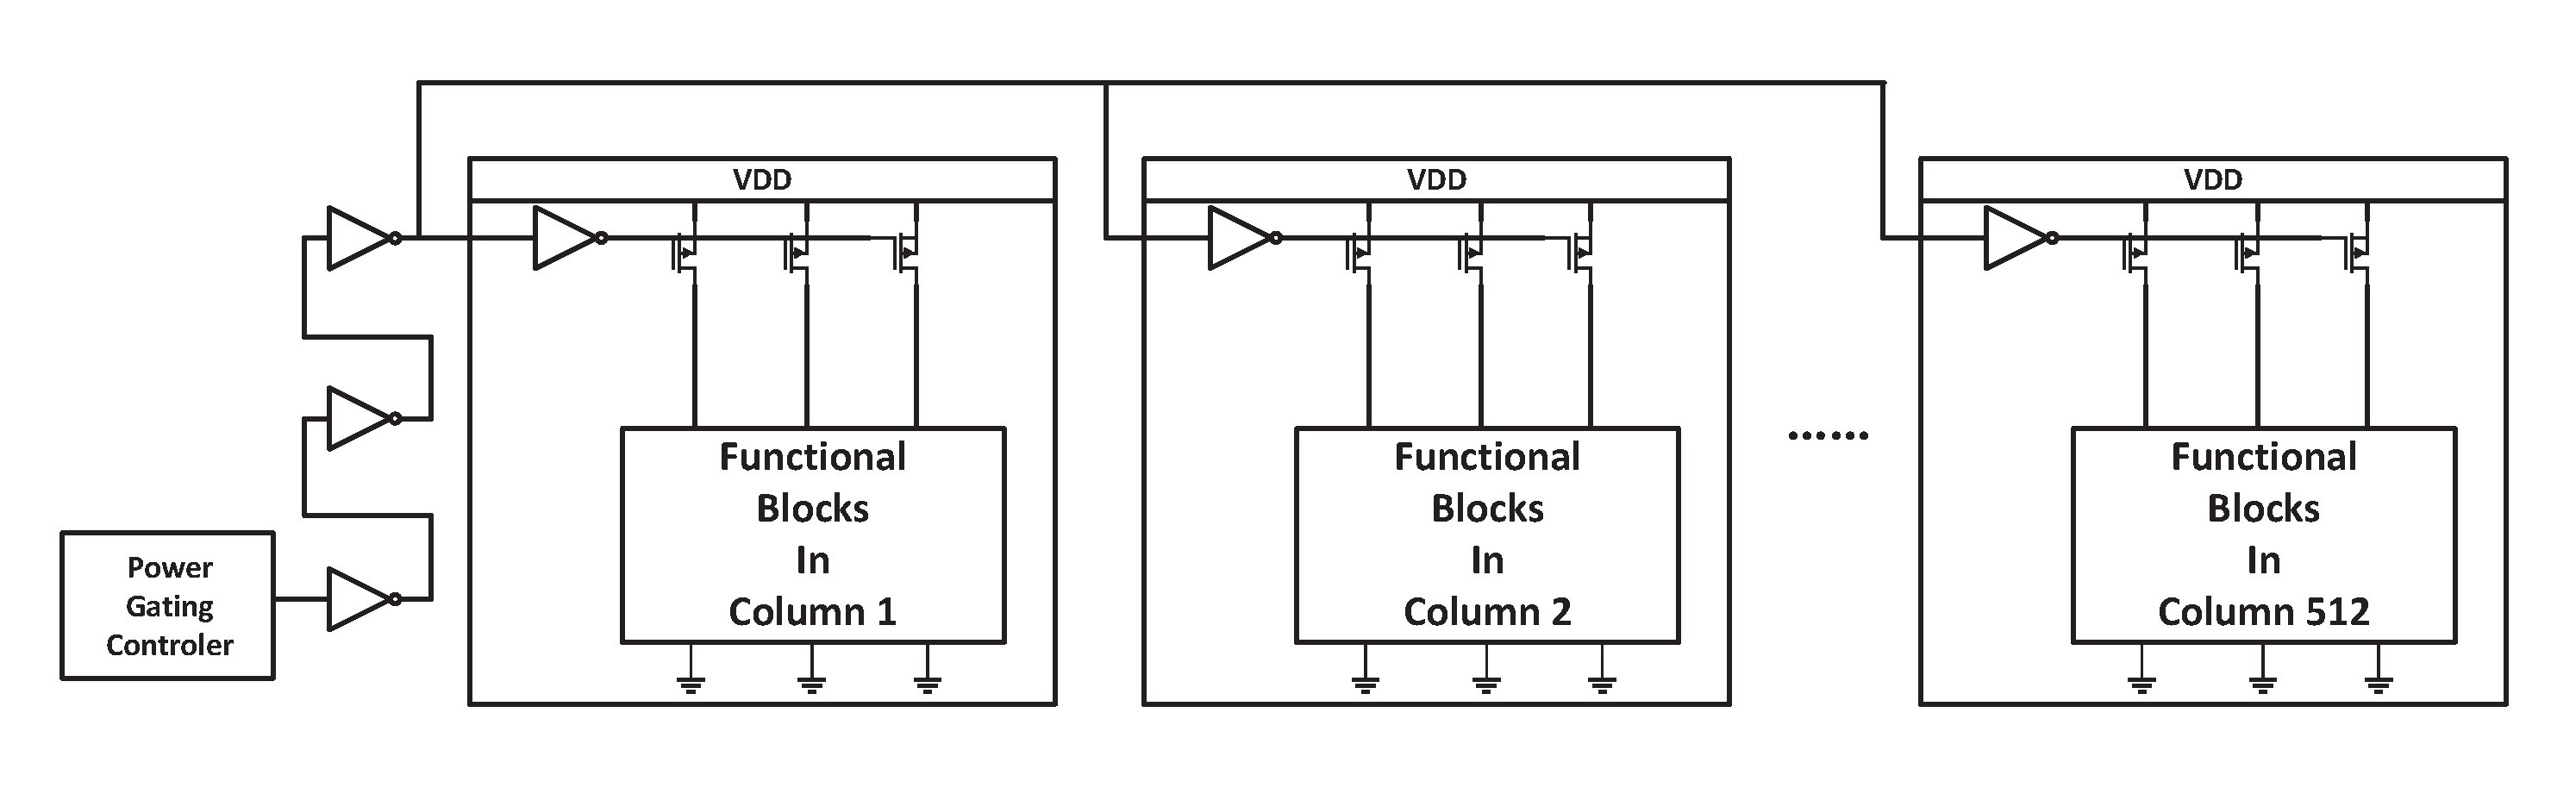
\includegraphics[width=3.5in]{./Figures/GATING.eps}}
	\caption{Implementation of power gating.}
	\label{GATING}
\end{figure} 

\begin{figure}[htbp]
	\centerline{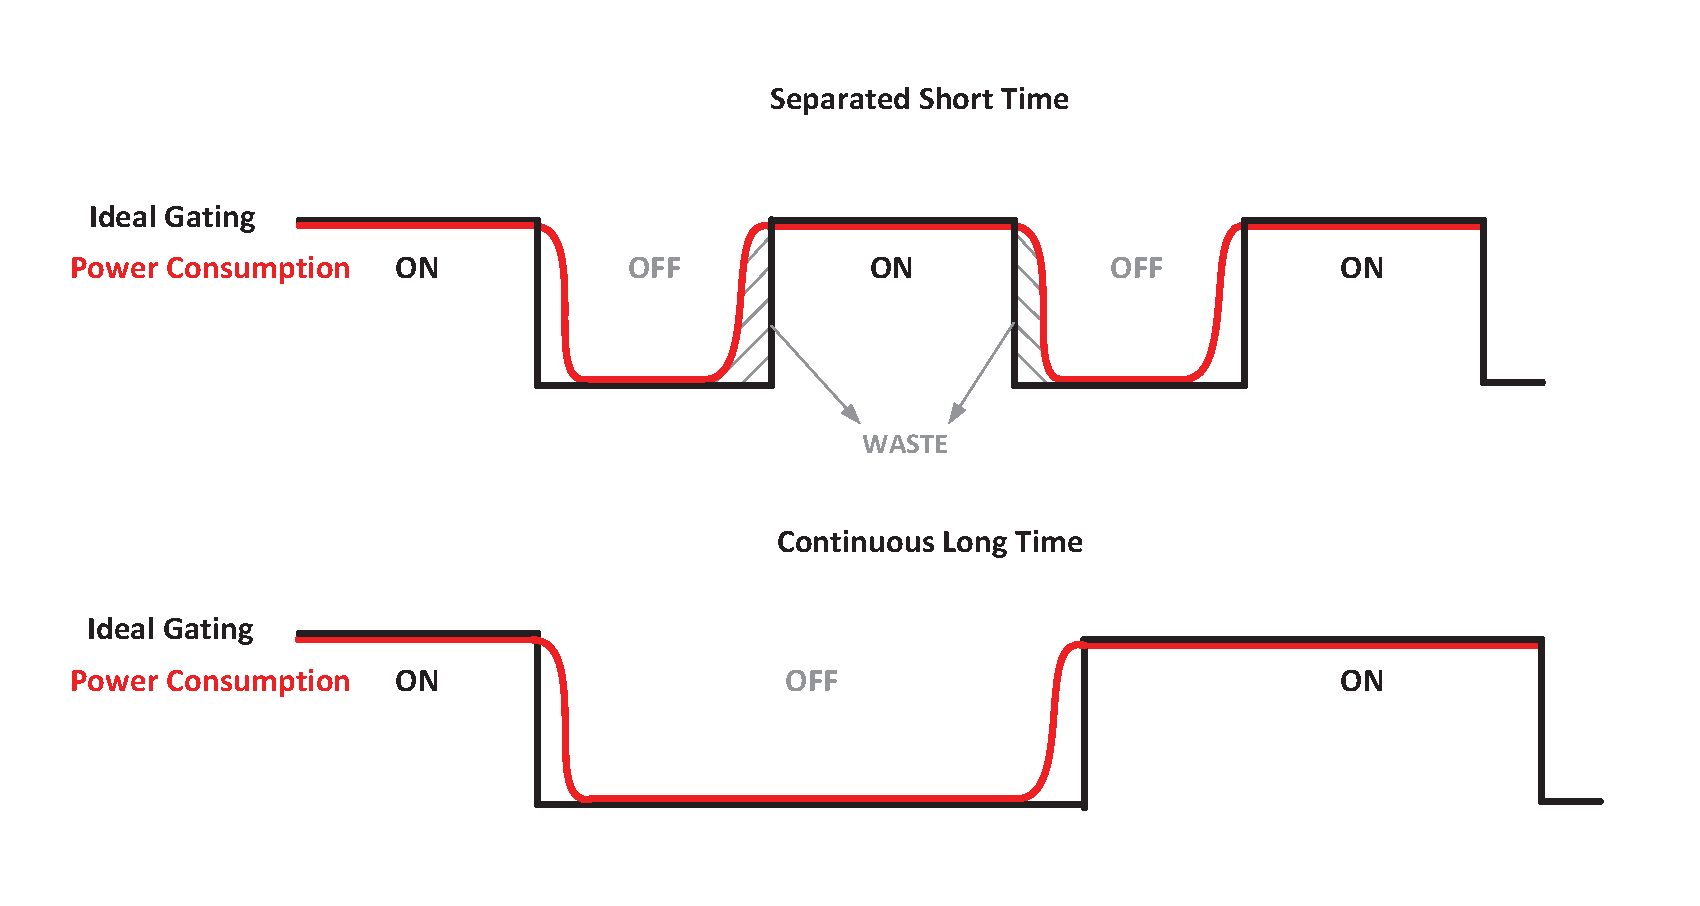
\includegraphics[width=3.5in]{./Figures/TIME.eps}}
	\caption{Continuous long time versus separated short time for power gating.}
	\label{TIME}
\end{figure}  

\subsection{Adaptive-Precision Implementation for the SS ADC}\label{gating2}

As evaluated in Sect.~\ref{result}, the SS ADC’ power consumption is mainly taken up by the column-parallel comparators, bias circuits, and the output buffer of the ramp generator. 
Considering that all bias circuits are settled down only once (tens of microseconds after the whole system's power up) and then other circuits can be settled down quickly by the distributed 
bias circuits, we just apply power gating to the amplifiers in the comparators and the output buffer in the ramp generator.

For low-precision conversion, the thermometer-code counter should have been extended to support switching the capacitors in CDAC 16 by 16 instead of one by one and thereby the ramp signal can reach $V_{refh}$ in 16 steps (for 4 bits) instead of in 256 steps (for 8 bits). 
After the 16 steps, the comparators and the output buffer can be power off for an extended period of time, leaving the related signals decrease gradually.
The related waveform are presented in Fig.~\ref{SS_pg}. 

\begin{figure}[htbp]
	\centerline{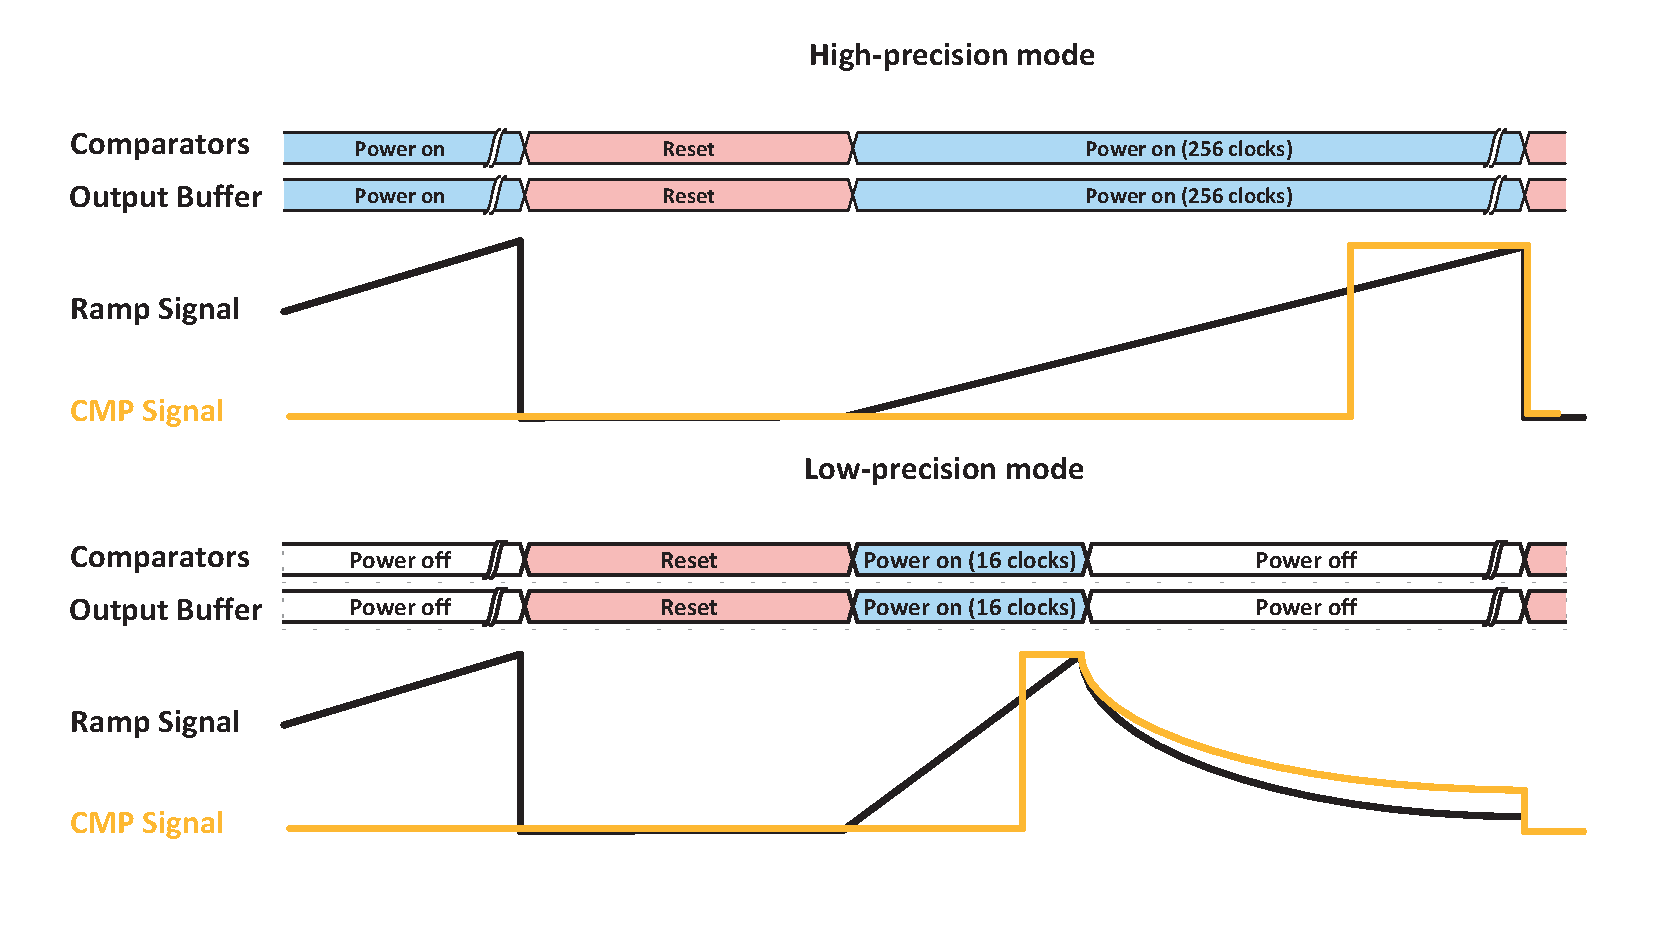
\includegraphics[width=3.2in]{./Figures/SS_pg.eps}}
	\caption{Adaptive-precision and power gating implementation for the SS ADC.}
	\label{SS_pg}
\end{figure} 

To avoid the decreasing output of comparators causing extra unwanted latch for the low-precision conversion results, an NMOS switch and a PMOS switch are inserted into the two inverters following the comparator as presented in Fig.~\ref{MATE}. 
For high-precision conversion, the gating signal will be low-level and turn on the PMOS switch, thus the second inverter's output will be the same as the comparator's output, which is either low-level or high-level. 
For low-precision conversion, the NMOS switch is turned on by the high-level gating signal and the second inverter's input is connected to the ground. Therefore, the output signal of the two inverters will remain high-level, preventing unpredictable latch caused by the comparator's metastable output.

\begin{figure}[htbp]
	\centerline{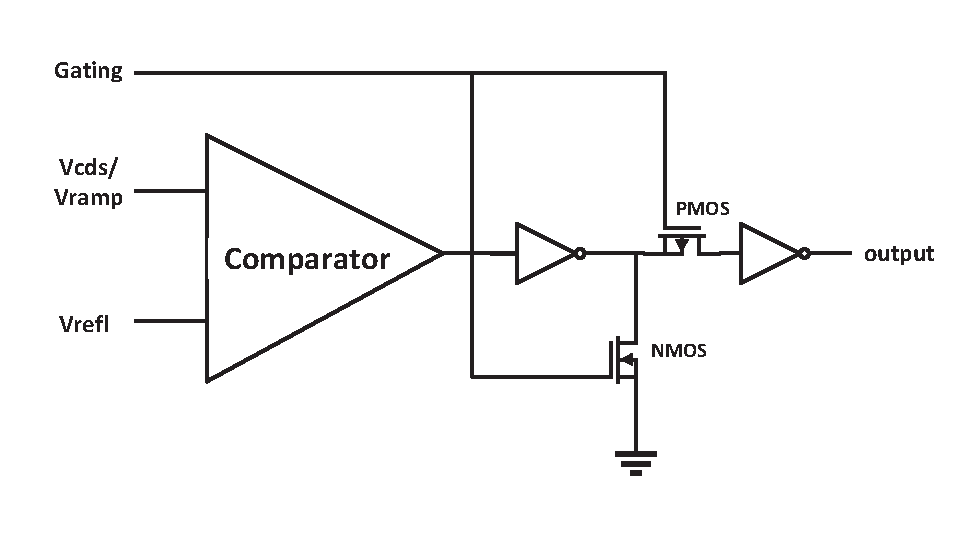
\includegraphics[width=2.5in]{./Figures/MATE.eps}}
	\caption{Two switches added to the inverters following the comparator in the SS ADC.}
	\label{MATE}
\end{figure} 

\subsection{Adaptive-Precision Implementation for the SAR/SS ADC}\label{gating3}

As evaluated in Sect.~\ref{result}, the SAR/SS ADC’ power consumption is mainly taken up by the column-parallel buffers of reference voltages in the SAR sub-ADC.
It is because that these buffers need to drive relatively large and changing load capacitance, which means relatively large static and dynamical current is required.
Therefore, gating these buffers will significantly reduce both static power consumption and dynamical power consumption for the ADC.

In addition, the CDS circuits and comparators in the SAR/SS ADC also consume a certain amount of energy. However, we only choose to take the comparators under control because they can conveniently share the same gating signal as the buffers'. And the gating signal of the buffers can also be the same as the start signal of the ramp generator. Therefore, gating the buffers and comparators in the SAR/SS ADC costs little extra control logic but some shared level-shifters and inverters.

Besides, the power distribution results in Sect.~\ref{result} shows that adaptive-precision tuning is not necessary within the ramp generator of the SAR/SS ADC, which means the counter in the SAR/SS ADC do not need to support two modes for adaptive-precision as in the SS ADC.

The waveform of related signals is presented in Fig.~\ref{SAR_pg}. It is noticed that For low-precision conversion, the ramp signal is generated as usual but the buffers and comparators will be power off, leaving the 4-bit results converted completely by the SAR logic. 

\begin{figure}[htbp]
	\centerline{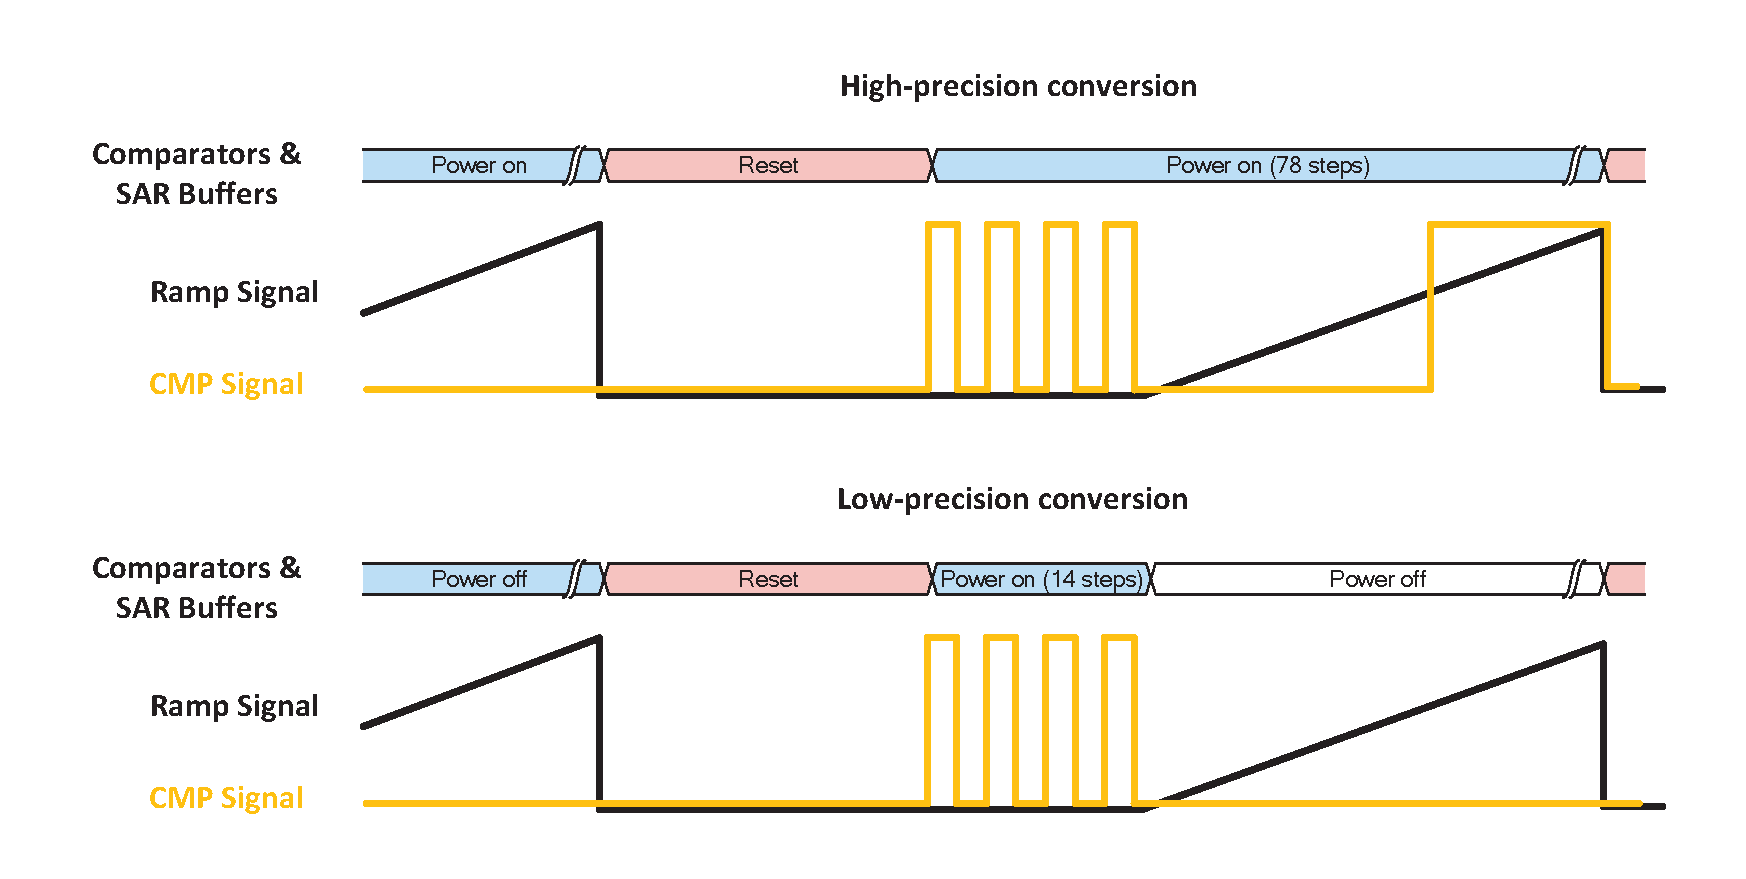
\includegraphics[width=3.5in]{./Figures/SAR_pg.eps}}
	\caption{Adaptive-precision and power gating implementation for the SAR/SS ADC.}
	\label{SAR_pg}
\end{figure} 
